\documentclass[11pt]{article}


\usepackage{preamble}

\title{Error Correcting Codes, Hardness Amplification and Boosting.}
\date{}

\begin{document}
    
\noindent Error Correcting Codes, Hardness Amplification and Boosting \hfill  CS 250, Winter 2025\\
\hrule

\section{Introduction}

\section{Preliminaries}

\section{Hardness Amplification with ECCs}

\begin{definition}{3.x}
    We say that a function $G : \pmo^\ell \rightarrow \pmo^{n}$ is an $(\ell, n)$-PRG if, for any size $n$ circuit $C$ over $n$ inputs, 
    \begin{equation*}
        \left|\Pr_{x \backsim U_n}[C(x)] - \Pr_{x \backsim U_s}[C(G(s))]\right| < \frac{1}{10}.
    \end{equation*}
\end{definition}

The parameter $\ell$ is the seed length.

\begin{assumption}{1} \label{a-1}
    There exists a function $f : \pmon \rightarrow \pmo$ such that $f$ can be computed in time $2^{O(n)}$, but there exists some $\delta > 0$ such that 
    \begin{equation*}
        \Corr\left(f, 2^{\delta n}\right) < 1.
    \end{equation*}
\end{assumption}

\begin{assumption}{2} \label{a-2}
    There exists a function $f : \pmon \rightarrow \pmo$ such that $f$ can be computed in time $2^{O(n)}$, but there exists some $\delta > 0$ such that 
    \begin{equation*}
        \Corr\left(f, 2^{\delta n}\right) < .9.
    \end{equation*}
\end{assumption}

\begin{assumption}{3} \label{a-3}
    There exists a function $f : \pmon \rightarrow \pmo$ such that $f$ can be computed in time $2^{O(n)}$, but there exists some $\delta > 0$ such that 
    \begin{equation*}
        \Corr\left(f, 2^{\delta n}\right) < 2^{-\Omega(n)}.
    \end{equation*}
\end{assumption}

We will prove that, given a worst case hard function $f$, we can transform it into an average case $f'$.

\begin{theorem}{3.x} If there exists a function $f$ satisfying the worst case hardness assumption, there exists a function $f'$ satisfying the average case hardness assumption.

\end{theorem}

\subsection{Why Hardness Amplification?}

\begin{theorem}{3.x} Suppose that $G$ is a $(O(\log n), n)$-PRG computable in $\poly(n)$ time. Then $\P = \BPP$.
\end{theorem}

\subsubsection{A Simple PRG}

\begin{theorem}{3.x}
    Given the average case hardness assumption, there exists a $(n - 1, n)$-PRG.
\end{theorem}

\subsubsection{The Nisan-Wigderson Generator}

\begin{theorem}{3.x}
    Given the average case hardness assumption, there exists a $(O(\log n), n)$-PRG.
\end{theorem}

\begin{center}
    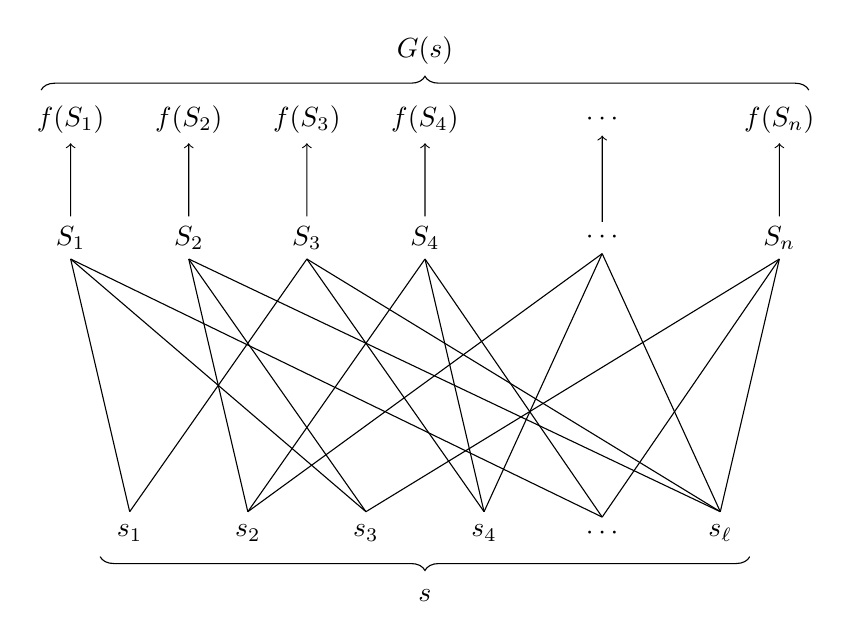
\begin{tikzpicture}[align=center,node distance=4cm, scale=1.5]
        \node[circle, inner sep=0pt, minimum size=15pt] (1) at (1, 0) {$s_1$}; 
        \node[circle, inner sep=0pt, minimum size=15pt] (2) at (2, 0) {$s_2$};
        \node[circle, inner sep=0pt, minimum size=15pt] (3) at (3, 0) {$s_3$};
        \node[circle, inner sep=0pt, minimum size=15pt] (4) at (4, 0) {$s_4$};
        \node[] (5) at (5, 0) {$\cdots$};
        \node[circle, inner sep=0pt, minimum size=15pt] (6) at (6, 0) {$s_{\ell}$};

        \node[] (11) at (.5, 2.5) {$S_1$};
        \draw[] (1.north) -- (11.south);
        \draw[] (3.north) -- (11.south);
        \draw[] (5.north) -- (11.south);

        \node[] (21) at (.5, 3.5) {$f(S_1)$};

        \draw[->] (11) -- (21);


        \node[] (12) at (1.5, 2.5) {$S_2$};
        \draw[] (2.north) -- (12.south);
        \draw[] (3.north) -- (12.south);
        \draw[] (6.north) -- (12.south);

        \node[] (22) at (1.5, 3.5) {$f(S_2)$};

        \draw[->] (12) -- (22);


        \node[] (13) at (2.5, 2.5) {$S_3$};
        \draw[] (1.north) -- (13.south);
        \draw[] (4.north) -- (13.south);
        \draw[] (6.north) -- (13.south);

        \node[] (23) at (2.5, 3.5) {$f(S_3)$};

        \draw[->] (13) -- (23);


        \node[] (14) at (3.5, 2.5) {$S_4$};
        \draw[] (2.north) -- (14.south);
        \draw[] (4.north) -- (14.south);
        \draw[] (5.north) -- (14.south);

        \node[] (24) at (3.5, 3.5) {$f(S_4)$};

        \draw[->] (14) -- (24);


        \node[] (15) at (5, 2.5) {$\cdots$};
        \draw[] (4.north) -- (15.south);
        \draw[] (2.north) -- (15.south);
        \draw[] (6.north) -- (15.south);

        \node[] (25) at (5, 3.5) {$\cdots$};

        \draw[->] (15) -- (25);

        \node[] (16) at (6.5, 2.5) {$S_n$};
        \draw[] (3.north) -- (16.south);
        \draw[] (5.north) -- (16.south);
        \draw[] (6.north) -- (16.south);

        \node[] (26) at (6.5, 3.5) {$f(S_n)$};

        \draw[->] (16) -- (26);

        \draw [decorate,decoration={brace,amplitude=5pt}]
  (0.25,3.75) -- (6.75,3.75) node[midway, yshift=.5cm]{$G(s)$};

        \draw[decorate, decoration={brace,amplitude=5pt, mirror}] 
        (.75, -.2) -- (6.25, -.2) node[midway, yshift=-.5cm]{$s$};
    \end{tikzpicture}
\end{center}

\subsection{Worst Case Hardness to Mild Hardness}

\newpage

\begin{theorem}{3.x}
    Suppose that $\cC$ is an $[m^2, m, .1]_2$ code which is computable in $\poly(m)$ time and locally decodable in $\polylog (m)$ time. Then if $f$ satisfies the worst case hardness assumption, $\cC \concat f$ satisfies the mild hardness assumption.
\end{theorem}

\begin{proof}
    Suppose that $f : \pmon \rightarrow \pmo$ satisfies the worst case hardness assumption, so that $f$ can be computed in time $2^{O(n)}$ yet, for some $\delta > 0$, $\Corr(f, 2^{\delta n}) < 1$. Writing $N = 2^n$, we can encode $f$ as a string $\TT(f) \in \pmo^{N}$ as its truth table. Then encoding $\TT(f)$ using $\cC$ to a string of length $N^2 = 2^{2n}$, we get can view this as a truth table for a function $\hat{f} : \pmo^{2n} \rightarrow \pmo$. We claim that if $f$ satisfies the worst case hardness assumption, $\hat{f}$ satisfies the mild hardness assumption. To prove that $\Corr(\hat{f}, 2^{n\delta/2}) \leq .9$, suppose for the sake of contradiction that $C$ is a circuit of size $2^{n \delta /2}$ with $\Corr(\hat{f}, C) > .9$. We will use this $C$ to construct a circuit $C'$ of size $S$ compute our original $f$ perfectly. First, consider the truth table $\TT(C)$ of the function computed by the circuit $C$. Because $\Corr(\hat{f}, C) > .9$, the string $\TT(C)$ and $\TT(\hat{f})$ have relative distance $\delta(\TT(C), \TT(\hat{f})) < .05$, which is less than half the distance of the code $\cC$. Since $\TT(\hat{f})$ is the encoding of $\TT(f)$ under the code $\cC$, we can recover $\TT(f)$ from $\TT(C)$.

    Suppose that $\LDec$ is the local decoder for $\cC$ running in $\polylog(N) = \poly(n)$ time. Consider the following randomized circuit $C_{\sfrac{2}{3}}$ for computing $f(x)$.

    \parbox{.4\linewidth}{%
        \begin{center}
            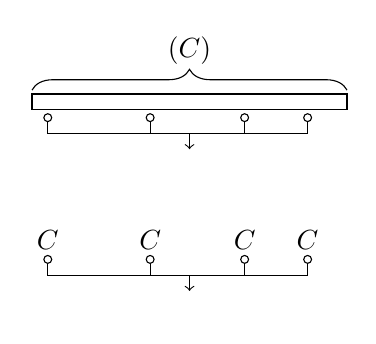
\begin{tikzpicture}

                \draw [decorate,decoration={brace,amplitude=7.5pt}]
        (0, .15) -- (4, 0.15) node[midway, yshift=.5cm]{$\TT(C)$};

                \draw[] (0, -.1) rectangle (4, .1);

                \draw[] (.2, -.2) -- (.2, -.4) -- (2, -.4);
                \draw[fill=white] (.2, -.2) circle (.05cm);
                \draw[] (1.5, -.2) -- (1.5, -.4);
                \draw[fill=white] (1.5, -.2) circle (.05cm);
                \draw[] (3.5, -.2) -- (3.5, -.4) -- (2, -.4);
                \draw[fill=white] (3.5, -.2) circle (.05cm);
                \draw[] (2.7, -.2) -- (2.7, -.4);
                \draw[fill=white] (2.7, -.2) circle (.05cm);

                \draw[->] (2, -.4) -- (2, -.6);

                \node[] at (2, -.8) {$\LDec$};

                

                \draw[] (.2, -2) -- (.2, -2.2) -- (2, -2.2);
                \draw[fill=white] (.2, -2) circle (.05cm);
                \node[] at (.2, -1.75) {$C$};
                \draw[] (1.5, -2) -- (1.5, -2.2);
                \draw[fill=white] (1.5, -2) circle (.05cm);
                \node[] at (1.5, -1.75) {$C$};
                \draw[] (3.5, -2) -- (3.5, -2.2) -- (2, -2.2);
                \draw[fill=white] (3.5, -2) circle (.05cm);
                \node[] at (3.5, -1.75) {$C$};
                \draw[] (2.7, -2) -- (2.7, -2.2);
                \draw[fill=white] (2.7, -2) circle (.05cm);
                \node[] at (2.7, -1.75) {$C$};

                \draw[->] (2, -2.2) -- (2, -2.4);

                \node[] at (2, -2.6) {$\LDec$};
            \end{tikzpicture}
        \end{center}
    }
    \hfill
    \parbox{.5\linewidth}{%
        \textbf{Input:} $x \in \pmo^n$
        \begin{enumerate}
            \item Compute $i$ such that $x$ is the $i$-th evaluation point in the truth table of $f$.
            \item Return $\LDec^{\TT(C)}(i)$ using $C$ to simulate queries to $\TT(C)$.
        \end{enumerate}
    }

    The size of $C_{\sfrac{1}{3}}$ is determined by the running time of $\LDec$ and the number of queries it makes to $\TT(C)$, both of which are polynomial in $n$. For each query that the local decoder $\LDec$ makes to $\TT(C)$, we'll need a copy of $C$ to compute this entry in the truth table; thus, the total size of $C_{\sfrac{1}{3}}$ is 
    \begin{equation*}
        |C_{\sfrac{1}{3}}| = \poly(n) \cdot |C| + \poly(n).
    \end{equation*}
    By the guarantees of our local decoding algorithm, for any input $x \in \pmon$, $\Pr[C_{\sfrac{1}{3}}(x) \neq f(x)] \leq \sfrac{1}{3}$, where this probability is over the random bits used by $C_{\sfrac{1}{3}}$. Since our goal is to compute $f$ perfectly, we can amplify the success probability by taking the majority over $O(n)$ copies of $C_{\sfrac{1}{3}}$ using independent random bits. This yields a circuit $C_{2^{-n}}$ of size $O(n \cdot |C_{\sfrac{1}{3}}|)$ such that $\Pr[C_{2^{-n}}(x) \neq f(x)] < 2^{-n}$. For a given setting of random bits $r$, write $C_{2^{-n}}^{(r)}$ to be a deterministic copy of $C_{2^{-n}}$ with fixed random bits. Then we can apply the union bound find to see
    \begin{equation*}
        \Pr_r\left[C^{(r)}_{2^{-n}}(x) = f(x) \text{ for all $x$}\right] \geq 1 - \sum_{x \in \pmon} \Pr_r\left[C^{(r)}_{2^{-n}}(x) = f(x)\right] > 1 - 2^{n} \cdot 2^{-n} = 0.
    \end{equation*}
    Thus, there must exist a particular $r$ such that $C^{(r)}_{2^{-n}}$ computes $f$ exactly. Note that the size of this circuit is 
    \begin{equation*}
        \left|C^{(r)}_{2^{-n}}\right| \leq O\left(n \cdot \poly(n) \cdot |C|\right) = \poly(n) \cdot 2^{\delta n / 2} \leq 2^{\delta n}.
    \end{equation*}
    However, this contradicts the fact that $\Corr(f, 2^{\delta n}) < 1$. Thus, $\Corr(\hat{f}, 2^{n\delta / 2}) \leq .9$. Note also that $\hat{f}$ will still be computable in time $2^{O(n)}$. Thus $\hat{f}$ satisfies the mild hardness assumption.
\end{proof}

Thus, we have reduced the task of hardness amplification to finding a suitable error correcting code. In class, we have seen two locally correctable codes: Reed-Muller codes and Hadamard codes. As a reminder, here are the definitions and parameters of those two codes:

\begin{definition}{3.x}[Reed-Muller Codes]
    Suppose $\F$ is a finite field of size $q$. The Reed-Muller code $\RM_q(m, r)$ is the set of all evaluations of $r$-degree $m$-variate polynomials over $\F_q$,
    \begin{equation*}
        \RM_q(m ,r) = \left\{(f(\gamma_1), f(\gamma_2), \ldots, f(\gamma_{q^m})) : f \in \F_q[X_1, \ldots, X_m], \, \deg (f) \leq r\right\},
    \end{equation*}
    where $\gamma_1, \ldots, \gamma_{q^m}$ is a canonical ordering of $\F_q^m$. This code has dimension $k = \binom{m + r}{r}$, block length $n = q^m$, and distance $d = 1 - r / q$.
\end{definition}

Suppose we set $r = .9q$ and $m = O(q / \log q)$.

\begin{definition}{3.x}[Hadamard Codes]

    
\end{definition}


\begin{definition}{3.x}
    The code $\cC$ will be the concatentation of a Reed-Solomon code $\RS$ with ... and a Hadamard Code
\end{definition}

\begin{center}
    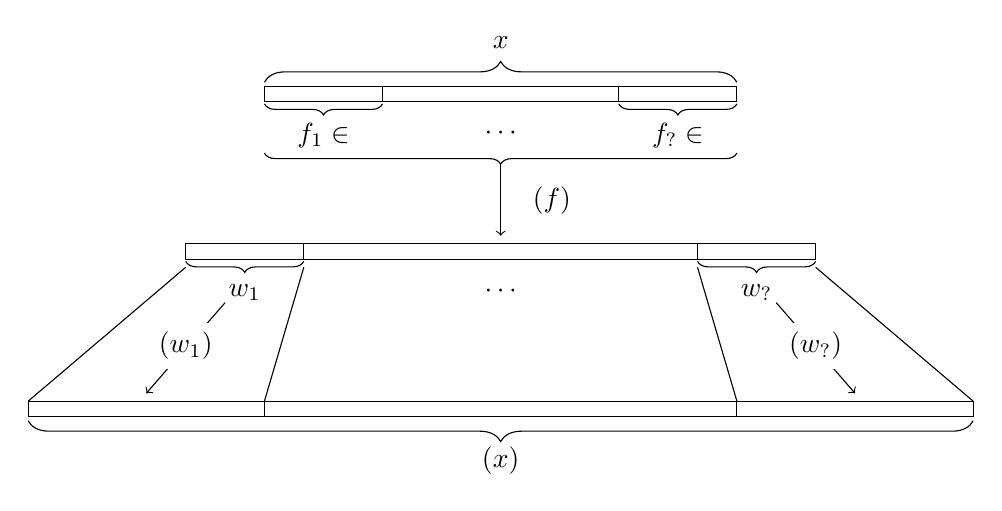
\begin{tikzpicture}

        % first row
        \draw [decorate,decoration={brace,amplitude=7.5pt}]
        (-3, 0.15) -- (3, 0.15) node[midway, yshift=.5cm]{$x$};

        \draw[] (-3, -.1) rectangle (3, .1);

        \draw[] (-1.5, -.1) -- (-1.5, .1);
        \draw [decorate,decoration={brace,amplitude=4pt, mirror}]
        (-3, -.125) -- (-1.5, -.125) node[midway, yshift=-.4cm]{$f_1 \in \F$};
        
        \node[] at (0, -.5) {$\cdots$};

        \draw[] (1.5, -.1) -- (1.5, .1); 
        \draw [decorate,decoration={brace,amplitude=4pt, mirror}]
        (1.5, -.125) -- (3, -.125) node[midway, yshift=-.4cm]{$f_? \in \F$};

        \draw [decorate,decoration={brace,amplitude=4pt, mirror}]
        (-3, -.75) -- (3, -.75);

        \draw[->] (0, -.9) -- (0, -1.8);
        \node[] at (.65, -1.35) {$\RM(f)$};
    
        % second row
        \draw[] (-4, -2.1) rectangle (4, -1.9);

        \draw[] (-2.5, -2.1) -- (-2.5, -1.9);

        \draw [decorate,decoration={brace,amplitude=4pt, mirror}]
        (-4, -2.125) -- (-2.5, -2.125) node[midway, yshift=-.4cm]{$w_1$};

        \draw[] (-4, -2.2) -- (-6, -3.9);
        \draw[] (-2.5, -2.2) -- (-3, -3.9);

        \draw[->] (-3.5, -2.65) -- (-4.5, -3.8);

        \node[fill=white] at (-4, -3.2) {$\Had(w_1)$};

        \node[] at (0, -2.5) {$\cdots$};

        \draw[] (2.5, -2.1) -- (2.5, -1.9);

        \draw [decorate,decoration={brace,amplitude=4pt, mirror}]
        (2.5, -2.125) -- (4, -2.125) node[midway, yshift=-.4cm]{$w_?$};

        \draw[] (4, -2.2) -- (6, -3.9);
        \draw[] (2.5, -2.2) -- (3, -3.9);

        \draw[->] (3.5, -2.65) -- (4.5, -3.8);

        \node[fill=white] at (4, -3.2) {$\Had(w_?)$};

        % third row
        \draw[] (-6, -4.1) rectangle (6, -3.9);

        \draw[] (-3, -4.1) -- (-3, -3.9);

        \draw[] (3, -4.1) -- (3, -3.9);

        \draw [decorate,decoration={brace,amplitude=7.5pt, mirror}]
        (-6, -4.15) -- (6, -4.15) node[midway, yshift=-.5cm]{$\Enc(x)$};

    \end{tikzpicture}
\end{center}

\subsection{Worst Case Hardness to Average Case Hardness}

\begin{theorem}{3.x}
    The average case hardness assumption implies the worst case hardness assumption.
\end{theorem}



\section{Boosting and Hardness Amplification}

\subsection{Smooth Boosters and The Hardcore Theorem}

\begin{center}
    \begin{tikzpicture}
        \path[draw] (-6.5, -2) rectangle (-2.5, 2);
        \path[draw,use Hobby shortcut,closed=true, pattern=north east lines]
        (-4,.3) .. (-4.4,.4) .. (-5.6, -.3);
        \node[fill=white] at (-4.6, -.5) {$H_1$};
        \node[] at (-4.5, 2.35) {$C_1$};


        \path[draw] (-2, -2) rectangle (2, 2);
        \path[draw,use Hobby shortcut,closed=true, pattern=north east lines]
        (0,.3) .. (.4,1) .. (.6,1.6) .. (1.4,1.4) .. (1.6, .3);
        \node[fill=white] at (.9, .7) {$H_2$};
        \node[] at (0, 2.35) {$C_2$};

        \path[draw] (2.5, -2) rectangle (6.5, 2);
        \path[draw,use Hobby shortcut,closed=true, pattern=north east lines]
        (4,.3) .. (4.4,.5) .. (5.6, -.3);
        \node[fill=white] at (4.7, -.3) {$H_3$};
        \node[] at (4.5, 2.35) {$C_3$};

        \draw[decorate, decoration={brace,amplitude=5pt, mirror}] 
        (-6.75, -2.25) -- (6.75, -2.25) node[midway, yshift=-.5cm]{};

        \draw[->] (0, -2.4) -- (0, -2.8);

        \path[draw] (-2, -7) rectangle (2, -3);
        \path[draw,use Hobby shortcut,closed=true, pattern=north east lines]
        (-.1,-5) .. (.4,-4.4) .. (1.6, -4.7);
        \node[fill=white] at (.8, -5) {$H$};
    \end{tikzpicture}
\end{center}

\subsection{Boosting via the XOR Lemma}

\section{One Shot Boosting with ECCs}


\end{document}